\begin{greek}
\chapter{Συλλογή σκουπιδιών με καταμέτρηση αναφορών}\label{ch:refcnt}
Οι αλγόριθμοι που έχουμε εξετάσει μέχρι στιγμής είναι έμμεσοι:
κάθε ένας από αυτούς διασχίζει τον γράφο των αντικειμένων
ώστε να αναγνωρίσει τα ζωντανά αντικείμενα. Σε αυτό το κεφάλαιο
εξετάζουμε την τέταρτη και τελευταία θεμελιώδη τεχνική συλλογής
σκουπιδιών, αυτήν της καταμέτρησης αναφορών.  
Η \textbf{συλλογή σκουπιδιών με καταμέτρηση αναφορών}, η
οποία οφείλεται στον Collins \cite{DBLP:journals/cacm/Collins60},
δεν επισκέπτεται όλο το σωρό προκειμένου να εντοπίσει τα
ζωντανά αντικείμενα και να συμπεράνει πώς όλα τα υπόλοιπα
είναι σκουπίδια, αλλά επιδρά απευθείας στα αντικείμενα
καθώς αναφορές σε αυτά δημιουργούνται ή καταστρέφονται.

Η αλγόριθμος διατηρεί μια απλή αναλλοίωτη: ένα αντικείμενο
θεωρείται ζωντανό αν και μόνο αν ο αριθμός των αναφορών σε
αυτό είναι αυστηρά θετικός. Η συλλογή με καταμέτρηση αναφορών
συσχετίζει λοιπόν έναν μετρητή αναφορών με κάθε διαχειριζόμενο
αντικείμενο. Ο μετρητής αυτός συνήθως αποθηκεύεται σε ένα
πεδίο στην  επικεφαλίδα του αντικειμένου.

Ο αλγόριθμος \ref{alg:refcnt_1} αποτελεί την απλούστερη
εκδοχή της συλλογής με καταμέτρηση αναφορών. Η διαδικασία
\textproc{Write} αυξάνει το μετρητή αναφορών του νέου
αντικειμένου στο οποίο αναφέρεται ένας δείκτης και μειώνει
το μετρητή αναφορών του παλαιού αντικειμένου προς το οποίο
αυτός αναφερόταν. Η διαδικασία αυτή καλείται ακόμη και για
την ενημέρωση τοπικών μεταβλητών. Κατά την έξοδο μιας
διαδικασίας, τέλος, η \textproc{Write} καλείται για να
ενημερώσει με την τιμή \null τις τοπικές μεταβλητές αυτής.
Οι διαδικασίες \textproc{addReference} και \textproc{deleteReference}
αυξάνουν και μειώνουν αντίστοιχα το μετρητή αναφορών του
αντικειμένου ορίσματος τους. Μόλις ένας μετρητής αναφορών
ενός αντικειμένου μηδενισθεί, τότε πριν η μνήμη αυτού
απελευθερωθεί, μειώνονται κατά ένα οι μετρητές αναφορών
των αντικειμένων στα οποία δείχνουν τα πεδία δείκτες
του.

Η μέθοδος \textbf{Write} αποτελεί ένα παράδειγμα ενός φράγματος
εγγραφής. Για κάθε φράγμα εγγραφής, ο μεταγλωττιστής παράγει
μία ακολουθία κώδικα πριν και μετά την εγγραφή ενός δείκτη.
Όπως θα δούμε και αργότερα, τα φράγματα εγγραφής είναι
απαραίτητα στην περίπτωση που οι συλλέκτες δε θεωρούν τη
ζωντάνια ολόκληρου του γράφου αντικειμένων ατομικά ως προς
τον τροποποιητή. Οι ταυτόχρονοι καθώς και οι γενεαλογικοί
συλλέκτες αποτελούν παραδείγματα τέτοιων συλλεκτών. Σε κάθε
περίπτωση, τα φράγματα εγγραφής εγγυώνται τη διατήρηση της
αναλλοίωτης του εκάστοτε αλγορίθμου συλλογής.

\begin{algorithm}[H]
  \caption{Απλή καταμέτρηση αναφορών}
  \label{alg:refcnt_1}
  \begin{algorithmic}[1]
    \Function{New}{\null}
      \State $ref \gets$ \Call{allocate}{\null}
      \If{$ref = \textbf{null}$}
        \State error ``Out of memory!''
      \EndIf
      \State \Call{rc}{$ref$} $\gets 0$
      \State \Return{$ref$}
    \EndFunction
    \Statex
    \Procedure{write}{$src$, $i$, $ref$}
      \State \textbf{atomic}
      \State \Call{addReference}{$ref$}
      \State \Call{deleteReference}{$src[i]$}
      \State $src[i] \gets ref$
    \EndProcedure
    \Statex
    \Procedure{addReference}{$ref$}
      \If{$ref \neq \textbf{null}$}
        \State \Call{rc}{$ref$} $\gets$ \Call{rc}{$ref$} $+1$
      \EndIf
    \EndProcedure
    \Statex
    \Procedure{deleteReference}{$ref$}
      \If{$ref \neq \textbf{null}$}
        \State \Call{rc}{$ref$} $\gets$ \Call{rc}{$ref$} $-1$
        \If{\Call{rc}{$ref$} $=$ $0$}
          \ForAll{$fld \; \textbf{in} Pointers(ref)$}
            \State \Call{deleteReference}{$*fld$}
          \EndFor
          \State \Call{free}{$ref$}
        \EndIf
      \EndIf
    \EndProcedure
  \end{algorithmic}
\end{algorithm}

\section{Πλεονεκτήματα \& Μειονεκτήματα}
Υπάρχουν αρκετοί λόγοι για τους οποίους η συλλογή με καταμέτρηση
αναφορών αποτελεί ελκυστική επιλογή. Αρχικά, το κόστος της
διαχείρισης μνήμης κατανέμεται στις λειτουργίες εγγραφής του
τροποποιητή, χωρίς να απαιτείται η παύση της εκτέλεσης αυτού.
Η μνήμη ενός αντικειμένου απελευθερώνεται αμέσως μόλις δεν
υπάρχει καμία αναφορά προς αυτό, κάτι που καθιστά τον αλγόριθμο
κατάλληλο για λειτουργία σε εφαρμογές όπου ο σωρός είναι
σχεδόν γεμάτος. Αντίθετα, οι συλλέκτες με εξιχνίαση, χρειάζονται
κάποιο χώρο στο σωρό ώστε να λειτουργήσουν. Επιπρόσθετα,
καθώς η καταμέτρηση αναφορών επιδρά απευθείας στα αντικείμενα
προέλευσης και προορισμού των δεικτών, η τοπικότητα του συλλέκτη
δε μπορεί να είναι χειρότερη από την τοπικότητα του τροποποιητή.
Ακόμη η συλλογή με καταμέτρηση αναφορών μπορεί να υλοποιηθεί
χωρίς καμία βοήθεια από το σύστημα εκτέλεσης ή το μεταγλωττιστή,
καθώς δεν απαιτεί τη γνώση των ριζών του προγράμματος. Τέλος,
όπως παρατηρούν οι Rodrigues και Jones \cite{DBLP:conf/wdag/RodriguesJ96}
η καταμέτρηση αναφορών μπορεί να ανακτήσει μνήμη ακόμα και
αν κάποια του συστήματος δεν είναι προσβάσιμα, κάτι που έχει
μεγάλη σημασία σε κατανεμημένα συστήματα.

Για όλους τους παραπάνω λόγους, η συλλογή με καταμέτρηση
αναφορών έχει υιοθετηθεί από πολλά συστήματα λογισμικού,
ανάμεσα στα οποία περιλαμβάνονται: υλοποιήσεις γλωσσών
προγραμματισμού (αρχικές εκδόσεις Smalltalk και Lisp, awk,
perl, python), εφαρμογές όπως το Photoshop, συστήματα
διαχείρισης εγγράφων και συστήματα διαχείρισης αρχείων
λειτουργικών συστημάτων. Επίσης, βιβλιοθήκες για ασφαλή
ανάκτηση μνήμης αντικειμένων είναι διαθέσιμες για γλώσσες
των οποίων το πρότυπο δεν επιβάλλει (ακόμη) αυτόματη
διαχείριση μνήμης. Οι βιβλιοθήκες αυτές χρησιμοποιούν
έξυπνους δείκτες για την πρόσβαση σε αντικείμενα. Οι
έξυπνοι δείκτες υπερφορτώνουν κατασκευαστές και τελεστές
όπως η ανάθεση, είτε για να επιβάλλουν αποκλειστική ιδιοκτησία
στα αντικείμενα είτε για να παρέχουν καταμέτρηση αναφορών.
Ο Edelson \cite{DBLP:conf/iwmm/Edelson92} ωστόσο παρατηρεί
πώς οι έξυπνοι δείκτες έχουν διαφορετική σημασιολογία από
τους ``πρωτόγονους'' δείκτες που προσπαθούν να μοντελοποιήσουν.

Ωστόσο, τη συλλογή σκουπιδιών με καταμέτρηση αναφορών
χαρακτηρίζουν και διάφορα μειονεκτήματα.

Πρώτον, η καταμέτρηση αναφορών επιβάλλει ένα χρονικό κόστος
στον τροποποιητή. Σε αντίθεση με τους αλγορίθμους εξιχνίασης
που εξετάσαμε στα προηγούμενα κεφάλαια, η καταμέτρηση αναφορών
επανορίζει όλες τις λειτουργίες \textproc{Read} και
\textproc{Write} δεικτών προκειμένου να διαχειριστεί τους
μετρητές αναφορών. Ακόμη και μια απλή διάσχιση μιας λίστας
απαιτεί μία αύξηση και μία μείωση ενός μετρητή αναφοράς για
κάθε αντικείμενο αυτής. Από άποψη επίδοσης, η επιβάρυνση
λειτουργιών που ενημερώνουν καταχωρητές και κομμάτια της
στοίβας είναι απαγορευτική. Γι αυτόν ακριβώς το λόγο, ο
απλοϊκός αλγόριθμος που παρουσιάστηκε είναι πρακτικά μη
εφαρμόσιμος για χρήση σε ένα γενικού σκοπού υψηλών επιδόσεων
διαχειριστή μνήμης.

Δεύτερον, τόσο οι ενέργειες που αφορούν διαχείριση των μετρητών
αναφορών όσο και οι φορτώσεις και αποθηκεύσεις δεικτών πρέπει
να είναι ατομικές ώστε να αποφευχθούν καταστάσεις συναγωνισμού
μεταξύ των νημάτων του τροποποιητή οι οποίες θα μπορούσαν να
οδηγήσουν σε πρώιμη αποδέσμευση της μνήμης ενός αντικειμένου.
Η εξασφάλιση της ατομικότητας μόνο της λειτουργίας ενημέρωσης
του μετρητή αναφοράς δεν επαρκεί. Κάποιες βιβλιοθήκες έξυπνων
δεικτών απαιτούν ιδιαίτερα προσεκτική μεταχείριση προκειμένου
να αποφευχθούν οι καταστάσεις συναγωνισμού. Για παράδειγμα,
η βιβλιοθήκη έξυπνων δεικτών Boost για τη γλώσσα C++, η οποία
παρέχει και λειτουργίες καταμέτρησης αναφορών, νήματα που
εκτελούνται ταυτόχρονα μπορεί είτε να διαβάζουν τον ίδιο
μοιραζόμενο δείκτη ταυτόχρονα είτε να μεταβάλλουν διαφορετικά
στιγμιότυπα αυτού. Η βιβλιοθήκη εξασφαλίζει όμως την
ατομικότητα μόνο των λειτουργιών αύξησης/μείωσης του μετρητή
αναφορών. Ο συνδυασμός ανάγνωσης/εγγραφής ενός δείκτη με την
ενημέρωση ενός μετρητή αναφοράς δεν αποτελεί μία μοναδική
ατομική πράξη.

Τρίτον, η απλοϊκή μέτρηση αναφορών μετατρέπει λειτουργίες
ανάγνωσης-μόνο (read-only) σε λειτουργίες που απαιτούν εγγραφή
στη μνήμη (ώστε να ενημερωθούν οι μετρητές αναφορών). Όμοια,
απαιτείται η ανάγνωση και εγγραφή του παλαιού αντικειμένου
αναφοράς ενός δείκτη πριν αυτός αλλάξει τιμή. Αυτές οι εγγραφές
``μολύνουν'' τη μνήμη cache και επιφέρουν επιπλέον κίνηση μεταξύ
μνήμης και επεξεργαστή.

Τέταρτον, η συλλογή με καταμέτρηση αναφορών αδυνατεί να συλλέξει
κυκλικές δομές δεδομένων (δομές δεδομένων που περιλαμβάνουν
αναφορές στον εαυτό τους). Ακόμη και αν μία τέτοια δομή είναι
απομονωμένη στο γράφο των αντικειμένων (δεν υπάρχει δηλαδή
μονοπάτι προς αυτή από τις ρίζες), οι μετρητές αναφοράς των
συνιστωσών της δε θα μηδενισθούν ποτέ. Οι Bacon και Rajan
\cite{DBLP:conf/ecoop/BaconR01} διαπιστώνουν πώς αυτοαναφορικές
δομές (διπλά συνδεδεμένες λίστες, κυκλικές ουρές, δένδρα με
δείκτες προς τη ρίζα κ.ά.) απαντώνται συχνά στις εφαρμογές,
παρότι η συχνότητά τους μπορεί να ποικίλλει σημαντικά από
εφαρμογή σε εφαρμογή.

Πέμπτον, στη χειρότερη περίπτωση, ο αριθμός των αναφορών σε
ένα αντικείμενο μπορεί να ισούται με το πλήθος των αντικειμένων
του σωρού. Αυτό συνεπάγεται πώς ο μετρητής αναφορών θα
καταλαμβάνει μια ολόκληρη λέξη μνήμης. Λαμβάνοντας υπόψη την
διαπίστωση των Dieckmann και H{\"o}lzle
\cite{DBLP:conf/ecoop/DieckmannH99} και Blackburn
κ.ά. \cite{DBLP:conf/oopsla/BlackburnGHKMBDFFGHHJLMPSVDW06}
πώς το μέσο μέγεθος αντικειμένων στις αντικειμενοστραφείς
γλώσσες είναι μικρό (στη Java 20-64 bytes) καθώς το γεγονός
πώς τα κελιά cons στη Lisp χρειάζονται συνήθως 2-3 λέξεις,
η επιβάρυνση σε χώρο μπορεί να είναι σημαντική.

Τέλος, η συλλογή σκουπιδιών με καταμέτρηση αναφορών μπορεί
επίσης να προκαλέσει παύσεις. Τη στιγμή που διαγράφεται ο
δείκτης στην κεφαλή μιας μεγάλης δομής δεδομένων, η διαδικασία 
\textproc{deleteReference} θα πρέπει να ελευθερώσει αναδρομικά
τη μνήμη όλων των αντικειμένων απογόνων της ρίζας. Ο Boehm
\cite{DBLP:conf/popl/Boehm04} μάλιστα ισχυρίζεται πώς οι
παύσεις αυτές μπορεί ακόμα και να ξεπεράσουν τις αντίστοιχες
παύσεις από συλλέκτες εξιχνίασης.

Στη συνέχεια εξετάζουμε προηγμένους αλγορίθμους συλλογής
σκουπιδιών με καταμέτρηση αναφορών.

\section{Καταμέτρηση αναφορών με αναβολή}
Τα περισσότερα συστήματα υψηλών επιδόσεων με καταμέτρηση
αναφορών, όπως για παράδειγμα των Blackburn και McKinley
\cite{DBLP:conf/oopsla/BlackburnM03} χρησιμοποιούν την τεχνική
της \textbf{καταμέτρησης αναφορών με αναβολή}. Η συντριπτική
πλειοψηφία των φορτώσεων δεικτών αφορά τοπικές και προσωρινές
μεταβλητές, δηλαδή καταχωρητές και στοίβα. Οι Deutsch και
Bobrow \cite{DBLP:journals/cacm/DeutschB76} έδειξαν πώς μπορούν
να αποφευχθούν οι ενέργειες καταμέτρησης αναφορών που αφορούν
αυτές τις λειτουργίες, ενημερώνοντας το μετρητή ενός αντικειμένου
μόνο όταν ο δείκτης προς αυτό αποθηκεύεται στο πεδίο κάποιου
αντικειμένου του σωρού. Οι λειτουργίες καταμέτρησης αναφορών
που αφορούν καταχωρητές και τη στοίβα αναβάλλονται. Με την
τεχνική αυτή, οι μετρητές αναφορών των τοπικών μεταβλητών
παύουν να είναι αξιόπιστοι: δεν είναι πλέον ασφαλής η
αποδέσμευση ενός αντικειμένου αν ο μετρητής αναφορών του
είναι μηδενικός. Η ανακύκλωση των αντικειμένων σκουπιδιών
απαιτεί την περιοδική διόρθωση των μετρητών κατά τη διάρκεια
παύσεων. Ο Ungar \cite{DBLP:conf/sde/Ungar84} δείχνει πώς
οι παύσεις αυτές είναι σημαντικά μικρότερες σε σχέση με τις
αντίστοιχες ενός συλλέκτη με σήμανση και εκκαθάριση.

Ο αλγόριθμος~\ref{alg:refcnt_2} φορτώνει τις αναφορές σε
αντικείμενα χρησιμοποιώντας, την απλή, χωρίς φράγμα υλοποίηση
\textproc{Read} που ορίστηκε στο κεφάλαιο~\ref{ch:intro}.
Παρόμοια, οι ρίζες ενημερώνονται με αναφορές χρησιμοποιώντας
μία μη φραγμένη εντολή store. Αντίθετα, οι εγγραφές σε
αντικείμενα του σωρού πρέπει να είναι φραγμένες. Στην
περίπτωση αυτή, η αύξηση ενός μετρητή αναφοράς γίνεται
κανονικά ως συνήθως. Ωστόσο, αν η μείωση του μετρητή αναφορών
του αντικειμένου στο οποίο έδειχνε ένας δείκτης έχει ως
αποτέλεσμα το μηδενισμό του μετρητή, το φράγμα εγγραφής
\textproc{Write} προσθέτει το αντικείμενο (μια αναφορά σε
αυτό) σε ένα πίνακα μηδενικών μετρητών (μεταβλητή $zct$)
αντί να το απελευθερώσει αμέσως. Ο πίνακας αυτός μπορεί
να υλοποιηθεί με διαφόρους τρόπους, χρησιμοποιώντας ένα
bitmap όπως ο Baden \cite{baden1983low} ή ένα hashtable
όπως οι Deutsch και Bobrow \cite{DBLP:journals/cacm/DeutschB76}.
H ανακύκλωση ενός αντικειμένου με μηδενικό μετρητή αναφορών
σε αυτό το σημείο δεν είναι ασφαλής, καθώς ενδέχεται να
υπάρχει μια αναφορά σε αυτό από τη στοίβα του προγράμματος.
Διαισθητικά, ο πίνακας μηδενικών μετρητών περιλαμβάνει
αναφορές σε αντικείμενα με μηδενικό μετρητή αναφορών τα
οποία μπορεί όμως να είναι ζωντανά.

Ωστόσο, τα αντικείμενα σκουπίδια πρέπει κάποια στιγμή να
συλλεγούν αν θέλουμε το πρόγραμμα να μην ξεμείνει από μνήμη.
Περιοδικά, για παράδειγμα όταν ο εκχωρητής αποτύχει να
επιστρέψει μνήμη στη συνάρτηση \textproc{New}, διακόπτεται
η λειτουργία των νημάτων του τροποποιητή και τα αντικείμενα
του πίνακα μηδενικών μετρητών εξετάζονται ώστε να ελεγχθεί
εάν ο πραγματικός μετρητής αναφορών τους είναι μηδενικός.

\begin{algorithm}[H]
  \caption{Καταμέτρηση αναφορών με αναβολή}
  \label{alg:refcnt_2}
  \begin{algorithmic}[1]
    \Function{New}{\null}
      \State $ref \gets$ \Call{allocate}{\null}
      \If{$ref = \textbf{null}$}
        \State \Call{collect}{\null}
        \State $ref \gets$ \Call{allocate}{\null}
        \If{$ref = \textbf{null}$}
          \State error ``Out of memory!''
        \EndIf
      \EndIf
      \State \Call{rc}{$ref$} $\gets 0$
      \State \Call{add}{$zct$, $ref$}
      \State \Return{$ref$}
    \EndFunction
    \Statex
    \Procedure{write}{$src$, $i$, $ref$}
      \If{$src = Roots$}
        \State $src[i] \gets ref$
      \Else
        \State \textbf{atomic}
        \State \Call{addReference}{$ref$}
        \State \Call{remove}{$zct$, $ref$}
        \State \Call{deleteReferenceToZCT}{$src[i]$}
        \State $src[i] \gets ref$
      \EndIf
    \EndProcedure
    \Statex
    \Procedure{deleteReferenceToZCT}{$ref$}
      \If{$ref \neq \textbf{null}$}
        \State \Call{rc}{$ref$} $\gets$ \Call{rc}{$ref$} $-1$
        \If{\Call{rc}{$ref$} $= 0$}
          \State \Call{add}{$zct$, $ref$} \Comment{defer freeing}
        \EndIf
      \EndIf
    \EndProcedure
    \Statex
    \Procedure{collect}{\null}
      \State \textbf{atomic}
      \ForAll{$fld \; \textbf{in} \; Roots$} \Comment{mark the stacks}
        \State \Call{addReference}{$*fld$}
      \EndFor
      \State \Call{sweepZCT}{\null}
      \ForAll{$fld \; \textbf{in} \; Roots$} \Comment{unmark the stacks}
        \State \Call{deleteReferenceToZCT}{$*fld$}
      \EndFor
    \EndProcedure
    \Statex
    \Procedure{sweepZCT}{\null}
      \While{\textbf{not} \Call{isEmpty}{$zct$}}
        \State $ref \gets$ \Call{remove}{$zct$}
        \If{\Call{rc}{$ref$} $= 0$} \Comment{now reclaim garbage}
          \ForAll{$fld \; \textbf{in} \; Pointers(ref)$}
            \State \Call{deleteReference}{$*fld$}
          \EndFor
          \State \Call{free}{$ref$}
        \EndIf
      \EndWhile
    \EndProcedure
  \end{algorithmic}
\end{algorithm}

Ένα τέτοιο αντικείμενο μπορεί να είναι ζωντανό μόνο αν
αναφέρεται σε αυτό κάποια ρίζα του τροποποιητή. Ο απλούστερος
τρόπος ανακάλυψης τέτοιων αντικειμένων είναι η σάρωση των
ριζών και η σήμανση των αντικειμένων αυτών δια μέσου της
αύξησης των μετρητών αναφοράς τους. Σε αυτό το σημείο ο
συλλέκτης είναι σίγουρος πώς ένα αντικείμενο με μηδενικό
μετρητή αναφορών δεν είναι προσβάσιμο και άρα είναι σκουπίδι.
Πλέον μπορούμε να διατρέξουμε ξανά τον πίνακα μηδενικών
μετρητών, αποδεσμεύοντας τα αντικείμενα με μηδενικό μετρητή
αναφοράς ως συνήθως. Τέλος, οι λειτουργίες σήμανσης
αντιστρέφονται: διατρέχονται οι ρίζες του τροποποιητή και
μειώνεται κατά ένα οι μετρητές αναφορών των αντικειμένων
στα οποία πιθανώς δείχνουν. Αν ο μετρητής αναφορών ενός
αντικειμένου μηδενισθεί, αυτό καταχωρείται εκ νέου στον
πίνακα μηδενικών μετρητών.

Η καταμέτρηση αναφορών με αναβολή αφαιρεί το κόστος της
μεταχείρισης μετρητών αναφοράς των τοπικών μεταβλητών από
τον τροποποιητή. Ο Ungar \cite{DBLP:conf/sde/Ungar84} και
ο Baden \cite{baden1983low} έχουν ισχυρισθεί πώς μπορεί να
μειώσει το κόστος των τροποποιήσεων δεικτών έως και 80\%.
Δεδομένης της σημασίας της τοπικότητας, μπορούμε να υποθέσουμε
πώς το πλεονέκτημα της καταμέτρησης αναφορών με αναβολή έναντι
της απλοϊκής καταμέτρησης αναφορών όσον αφορά την επίδοση
θα είναι ακόμη μεγαλύτερο στο σύγχρονο υλικό. Ωστόσο, οι
επιδιορθώσεις των μετρητών αναφοράς λόγω ενημερώσεων πεδίων
δεικτών αντικειμένων πρέπει να πραγματοποιούνται πρόθυμα
και ατομικά.

\section{Καταμέτρηση αναφορών με συγκέντρωση}
Η καταμέτρηση αναφορών με αναβολή αφορά το κόστος της εφαρμογής
λειτουργιών καταμέτρησης αναφορών σε τοπικές μεταβλητές.
Το πρόβλημα του πώς να μειωθεί το κόστος από την καταμέτρηση
αναφορών που προκύπτει από την ενημέρωση δεικτών που
αποθηκεύονται σε πεδία αντικειμένων. Οι Levanoni και Petrank
\cite{levanoni1999scalable} παρατηρούν πώς, για κάθε χρονική
περίοδο και κάθε αντικείμενο, μόνο οι τιμές στην αρχή και
το τέλος της περιόδου έχουν σημασία και οι ενδιάμεσες τιμές
μπορούν να αγνοηθούν. Επομένως αρκετές καταστάσεις ενός
αντικειμένου μπορούν να συγκεντρωθούν σε αυτές τις δύο. Για
παράδειγμα, έστω ένα αντικείμενο X, οποίο περιλαμβάνει ένα
δείκτη $f$, ο οποίος αρχικά αναφέρεται στο αντικείμενο $O_0$
και ενημερώνεται συνέχεια ώστε να δείχνει στα αντικείμενα 
$O_1, O_2, \dots O_3$. Αυτό θα είχε ως αποτέλεσμα την ακόλουθη
αλληλουχία ενεργειών καταμέτρησης αναφορών:\\

rc($O_0$)--, rc($O_1$)++, rc($O_1$)--, rc($O_2$)++, ..., rc($O_n$)++.\\

Οι ενδιάμεσες λειτουργίες αλληλοαναιρούνται και μπορούν να
παραλειφθούν. Οι Levanoni και Petrank \cite{levanoni1999scalable} 
τις αγνοούν αντιγράφοντας αντικείμενα σε έναν τοπικό χώρο
καταγραφής πριν την πρώτη τροποποίηση του στη διάρκεια μιας
εποχής. Τη στιγμή που ενημερώνεται ο δείκτης ενός αντικειμένου,
αυτό καταχωρείται, δηλαδή η διεύθυνσή του και οι τρέχουσες
τιμές των δεικτών που περιέχει αποθηκεύονται σε έναν τοπικό
απομονωτή ενημέρωσης. Το τροποποιημένο αντικείμενο σημειώνεται
ως βρώμικο.

Η διαδικασία \textproc{log} επιχειρεί να αποφύγει την
παρουσία διπλών εγγραφών στον τοπικό χώρο καταχώρησης ενός
νήματος προσαρτώντας αρχικά τις τιμές των πεδίων δεικτών
του αντικειμένου στο χώρο καταγραφής. Στη συνέχεια αφού
ελέγξει πώς το αντικείμενο ακόμη δεν είναι βρώμικο,
οριστικοποιεί την καταγραφή γράφοντας το αντικείμενο στο
χώρο καταγραφής, σημειωμένο κατάλληλα ώστε να μπορεί να
αναγνωρισθεί ως καταγραφή αντικειμένου και όχι ως καταγραφή
πεδίου αντικειμένου. Τέλος, ενημερώνεται ο εσωτερικός δρομέας
του χώρου καταγραφής. Το αντικείμενο σημειώνεται ως βρώμικο
με την εγγραφή ενός δείκτη στην καταγραφή του στην επικεφαλίδα
του. 

\begin{algorithm}[H]
  \caption{Καταμέτρηση αναφορών με συγκέντρωση: φράγμα εγγραφής}
  \begin{algorithmic}[1]
    \State $me \gets myThreadId$
    \Statex
    \Procedure{Write}{$src$, $i$, $ref$}
      \State $ref \gets$ \Call{allocate}{\null}
      \If{\textbf{not} \Call{dirty}{$src$}}
        \State \Call{log}{$src$}
      \EndIf
      \State $src[i] \gets ref$
    \EndProcedure
    \Statex
    \Procedure{log}{$obj$}
      \ForAll{$fld \; \textbf{in} \; Pointers(obj)$}
        \If{$*fld \neq \textbf{null}$}
          \State \Call{append}{$updates[me]$, $*fld$}
        \EndIf
      \EndFor
      \If{\textbf{not} \Call{dirty}{$obj$}}
        \State $slot \gets$ \Call{appendAndCommit}{$updates[me]$, $obj$}
        \State \Call{setDirty}{$obj$, $slot$}
      \EndIf  
    \EndProcedure
    \Statex
    \Function{dirty}{$obj$}
      \State \Return{\Call{logPointer}{$obj$} $\neq CLEAN$}
    \EndFunction
    \Statex
    \Procedure{setDirty}{$obj$, $slot$}
      \State \Call{logPointer}{$obj$} $\gets slot$ \Comment{address of entry for obj in updates[me]}
    \EndProcedure
  \end{algorithmic}
\end{algorithm}

Παρότι μια κατάσταση συναγωνισμού μπορεί να οδηγήσει στην
καταγραφή του στιγμιοτύπου ενός αντικειμένου σε περισσότερους
του ενός τοπικούς απομονωτές, ο αλγόριθμος εγγυάται πώς οι
καταγραφές θα είναι πανομοιότυπες μεταξύ τους και επομένως
δεν έχει σημασία σε ποια από όλες δείχνει η επικεφαλίδα του
αντικειμένου. Ανάλογα βέβαια με το μοντέλο συνέπειας μνήμης
του επεξεργαστή, αυτό το φράγμα εγγραφής μπορεί να μην απαιτεί
λειτουργίες συγχρονισμού.

Στην αρχή κάθε κύκλου συλλογής, ο αλγόριθμος διακόπτει κάθε
νήμα του τροποποιητή, μεταφέρει τον απομονωτή ενημερώσεων
αυτού στο χώρο καταχώρισης του συλλέκτη και δεσμεύει ένα νέο
απομονωτή ενημερώσεων. Η διαδικασία \textproc{processReferenceCounts}
ελέγχει αν ένα αντικείμενο είναι ακόμη βρώμικο πριν ενημερώσει
τους μετρητές αναφορών. Οι μετρητές αναφορών των παιδιών ενός
αντικειμένου πριν την πρώτη του τροποποίηση στην τρέχουσα
εποχή μειώνονται, ενώ αντίστοιχα οι μετρητές αναφορών των
τρεχόντων παιδιών του αυξάνονται. Σε ένα απλό σύστημα, κάθε
αντικείμενο με μηδενικό μετρητή αναφορών θα μπορούσε να
αποδεσμευθεί αναδρομικά. Ωστόσο, αν η καταμέτρηση αναφορών
σε τοπικές μεταβλητές αναβάλλεται, ή αν για λόγους επίδοσης
ο αλγόριθμος δεν εγγυάται πώς θα διαχειριστεί όλες τις αυξήσεις
πριν τις μειώσεις, μπορούμε απλά να θυμηθούμε ένα αντικείμενο
με μηδενικό μετρητή αναφορών. Ο αλγόριθμος επίσης καθαρίζει
το αντικείμενο (αφαιρεί τη σήμανση dirty) ούτως ώστε αυτό να
μην επανεξεταστεί στη διάρκεια του τρέχοντος κύκλου συλλογής.
Οι δείκτες στα παλαιά παιδιά ενός αντικειμένου μπορούν να
βρεθούν από το στιγμιότυπο αυτού στο χώρο καταχώρησης, ενώ οι
δείκτες στα τρέχοντα παιδιά του από το αντικείμενο καθεαυτό.
Οι Paz και Petrank σημειώνουν \cite{DBLP:conf/cc/PazP07} πώς
υπάρχει η δυνατότητα για προφόρτωση αντικειμένων ή μετρητών
αναφορών κατά την εκτέλεση των βρόχων των διαδικασιών
\textproc{decrementOld} και \textproc{incrementNew}.

\begin{algorithm}[H]
  \caption{Καταμέτρηση αναφορών με συγκέντρωση: ενημέρωση μετρητών αναφορών}
  \label{alg:refcnt_4}
  \begin{algorithmic}[1]
    \Procedure{collect}{\null}
      \State \Call{collectBuffers}{\null}
      \State \Call{processReferenceCounts}{\null}
      \State \Call{sweepZCT}{\null}
    \EndProcedure
    \Statex
    \Procedure{collectBuffers}{\null}
      \State $collectorLog \gets []$
      \ForAll{$t \; \textbf{in} \; Threads$}
        \State $collectorLog \gets collectorLog + updates[t]$
      \EndFor
    \EndProcedure
    \Statex
    \Procedure{processReferenceCounts}{\null}
      \ForAll{$entry \; \textbf{in} \; collectorLog$}
        \State $obj \gets$ \Call{objFromLog}{$entry$}
        \If{\Call{dirty}{$obj$}} \Comment{do not process duplicates}
          \State \Call{logPointer}{$obj$} $\gets CLEAN$
          \State \Call{incrementNew}{$obj$}
          \State \Call{decrementOld}{$entry$}
        \EndIf
      \EndFor
    \EndProcedure
    \Statex
    \Procedure{decrementOld}{$entry$}
      \ForAll{$fld \; \textbf{in} \; Pointers(entry)$} \Comment{use the values in the collector's log}
        \State $child \gets *fld$
        \If{$child \neq \textbf{null}$}
          \State \Call{rc}{$child$} $\gets$ \Call{rc}{$child$} $-1$
          \If{\Call{rc}{$child$} $=0$}
            \State \Call{add}{$zct$, $child$}
          \EndIf
        \EndIf
      \EndFor
    \EndProcedure
    \Statex
    \Procedure{incrementNew}{$obj$}
      \ForAll{$fld \; \textbf{in} \; Pointers(obj)$} \Comment{use the values in the object}
        \State $child \gets *fld$
        \If{$child \neq \textbf{null}$}
          \State \Call{rc}{$child$} $\gets$ \Call{rc}{$child$} $+1$
        \EndIf
      \EndFor
    \EndProcedure
  \end{algorithmic}
\end{algorithm}  

Ο συνδυασμός της καταμέτρησης αναφορών με αναβολή και συγκέντρωση
αφαιρεί το κόστος της καταμέτρησης αναφορών από τον τροποποιητή.
Το πλεονέκτημα αυτό ωστόσο δεν έρχεται χωρίς κόστος. Έχουμε
επανεισάγει παύσεις στη λειτουργία του τροποποιητή (παρότι
αυτές αναμένεται να είναι συντομότερες από τις αντίστοιχες ενός
συλλέκτη εξιχνίασης) και επίσης αυξήσει τις απαιτήσεις σε μνήμη
για τη διατήρηση των απομονωτών και του πίνακα μηδενικών μετρητών.

\section{Κυκλική Καταμέτρηση Αναφορών}
Καθώς οι μετρητές αναφορών των αντικειμένων μιας κυκλικής δομής
δεδομένων είναι τουλάχιστον ένα, η απλή καταμέτρηση αναφορών
δεν μπορεί από μόνη της να συλλέξει τέτοιες δομές. Οι κύκλοι
ωστόσο εμφανίζονται συχνά και δημιουργούνται τόσο από τους
προγραμματιστές εφαρμογών όσο και το σύστημα εκτέλεσης.

\begin{figure}[H]
  \centering
  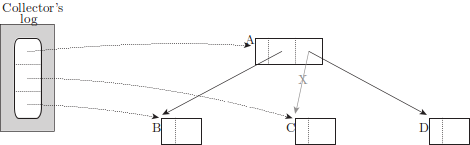
\includegraphics{figures/refcnt_1}
  \caption{Καταμέτρηση αναφορών με συγκέντρωση.}
  \label{fig:refcnt_1}  
\end{figure}

Η απλούστερη προσέγγιση στο πρόβλημα είναι ο συνδυασμός της
καταμέτρησης αναφορών με συνήθη, εφεδρική συλλογή εξιχνίασης.
Η ελπίδα είναι πώς τα περισσότερα αντικείμενα δε θα είναι 
προσβάσιμα από κύκλους και επομένως θα απελευθερώνονται
αμέσως από την καταμέτρηση αναφορών. Οι εναπομείνασες
κυκλικές δομές συλλέγονται από το συλλέκτη εξιχνίασης. Η
ιδέα αυτή απλά μειώνει τη συχνότητα εκτέλεσης της συλλογής
εξιχνίασης. Σε επίπεδο γλώσσας, οι Friedman και Wise
\cite{DBLP:journals/ipl/FriedmanW79} παρατήρησαν πώς κύκλοι
μπορούν να δημιουργηθούν μόνο σε αγνές συναρτησιακές γλώσσες
από αναδρομικούς ορισμούς και επομένως μπορούν να
αντιμετωπιστούν ειδικά δεδομένης της παρατήρησης ορισμένων
περιορισμών.

Πολλοί ερευνητές έχουν προτείνει την ειδική αντιμετώπιση
των λειτουργιών εγγραφής δεικτών που κλείνουν κύκλους.
Μεταξύ αυτών είναι οι Friedman και Wise,
\cite{DBLP:journals/ipl/FriedmanW79}, ο BrownBridge
\cite{DBLP:conf/fpca/Brownbridge85}, ο Salkild
\cite{salkild1987implementation}; o Pepels κ.ά.
\cite{pepels1988cyclic} καθώς και ο Axford
\cite{DBLP:journals/cj/Axford90}.

Οι πιο ευρέως υιοθετημένοι μηχανισμοί για το χειρισμό
κυκλικών δομών με καταμέτρηση αναφορών ωστόσο χρησιμοποιούν
μία τεχνική γνωστή και ως \textbf{δοκιμαστική διαγραφή}.
Η βασική ιδέα αφορά στο ότι δεν είναι απαραίτητο ο εφεδρικός
συλλέκτης εξιχνίασης να επισκεφτεί ολόκληρο τον γράφο των
ζωντανών αντικειμένων. Αντίθετα, αυτός μπορεί να εστιάσει
την προσοχή του σε εκείνα τα τμήματα του γράφου στα οποία
η διαγραφή ενός δείκτη μπορεί να δημιούργησε έναν κύκλο
σκουπιδιών. Ας παρατηρήσουμε πώς:

\begin{itemize}
  \item Σε κάθε κύκλο σκουπιδιών, οι μη μηδενικοί μετρητές
    αναφοράς οφείλονται σε εσωτερικούς δείκτες.
  \item Οι κύκλοι σκουπιδιών μπορεί να προκύψουν μόνο από τη
    διαγραφή κάποιου δείκτη που αφήνει το μετρητή αναφοράς
    κάποιου αντικειμένου θετικό.
\end{itemize} 

Οι αλγόριθμοι μερικής εξιχνίασης εκμεταλλεύονται τις παραπάνω
παρατηρήσεις επισκεπτόμενοι μόνο το υπογράφημα αντικειμένων
που έχει ως ρίζα κάποιο αντικείμενο το οποίο υποπτεύονται
πώς είναι σκουπίδι. Οι αλγόριθμοι αυτοί διαγράφουν δοκιμαστικά
κάθε δείκτη που συναντούν μέσω της μείωσης προσωρινά του
μετρητή αναφορών του αντικειμένου στο οποίο αυτός αναφέρεται.
Με τον τρόπο αυτό, πρακτικά αφαιρούν τη συμβολή των εσωτερικών
δεικτών στην κυκλικότητα της δομής. Αν ο μετρητής αναφορών ενός
αντικειμένου εξακολουθεί να είναι μη μηδενικός μετά από τη
διαδικασία αυτή, τότε αυτό θα πρέπει να είναι προσβάσιμο από
κάποιο αντικείμενο εκτός του υπογράφου και συνεπώς το αντικείμενο
δεν είναι σκουπίδι. Επιπλέον ούτε το μεταβατικό κλείσιμο του
αντικειμένου ως προς την προσβασιμότητα μέσω δεικτών περιέχει
σκουπίδια.

Ο Bacon κ.ά. \cite{DBLP:conf/pldi/BaconALRS01}, οι Bacon
και Rajan \cite{DBLP:conf/ecoop/BaconR01} και ο Paz κ.ά.
\cite{DBLP:journals/toplas/PazBKPR07} επινόησαν τον αλγόριθμο
Recycler που υποστηρίζει ταυτόχρονη κυκλική καταμέτρηση
αναφορών. Στην παρούσα φάση παρουσιάζουμε τη σύγχρονη εκδοχή
του αλγορίθμου, αναβάλλοντας την παρουσίαση της ασύγχρονης
για το κεφάλαιο 8. Ο αλγόριθμος~\ref{alg:refcnt_5} δρα σε
3 περάσματα:

\begin{algorithm}
  \caption{Κυκλική καταμέτρηση αναφορών: ο αλγόριθμος Recycler}
  \label{alg:refcnt_5}
  \begin{algorithmic}[1]
    \Function{New}{\null}
      \State $ref \gets$ \Call{allocate}{\null}
      \If{$ref = \textbf{null}$}
        \State \Call{collect}{\null} \Comment{the cycle collector}
        \State $ref \gets$ \Call{allocate}{\null}
        \If{$ref = \textbf{null}$}
          \State error ``Out of memory!''
        \EndIf
      \EndIf
      \State \Call{rc}{$ref$} $\gets 0$
      \State \Return{$ref$}
    \EndFunction
    \Statex
    \Procedure{addReference}{$ref$}
      \If{$ref \neq \textbf{null}$}
        \State \Call{rc}{$ref$} $\gets$ \Call{rc}{$ref$} $+1$
        \State \Call{colour}{$ref$} $\gets black$ \Comment{cannot be in a garbage cycle}
      \EndIf
    \EndProcedure
    \Statex
    \Procedure{deleteReference}{$ref$}
      \If{$ref \neq \textbf{null}$}
        \State \Call{rc}{$ref$} $\gets$ \Call{rc}{$ref$} $-1$
        \If{\Call{rc}{$ref$} $=0$}
          \State \Call{release}{$ref$}
        \Else
          \State \Call{candidate}{$ref$} \Comment{might isolate a garbage cycle}
        \EndIf
      \EndIf
    \EndProcedure
    \Statex
    \Procedure{release}{$ref$}
      \ForAll{$fld \; \textbf{in} \; Pointers(ref)$}
        \State \Call{deleteReference}{$fld$}
      \EndFor
      \State \Call{colour}{$ref$} $\gets black$ \Comment{objects on the free-list are black}
      \If{\textbf{not} $ref$ \textbf{in} $candidates$} \Comment{deal with candidates later}
        \State \Call{free}{$ref$}
      \EndIf
    \EndProcedure
    \Statex
    \Procedure{candidate}{$ref$} \Comment{colour as a candidate and add to the set}
      \If{\Call{colour}{$ref$} $\neq purple$}
        \State \Call{colour}{$ref$} $\gets purple$
        \State $candidates \gets candidates \cup {ref}$
      \EndIf
    \EndProcedure
    \Statex
    \Procedure{collect}{\null}
      \State \textbf{atomic}
      \ForAll{$ref \; \textbf{in} \; candidates$}
        \State \Call{scan}{$ref$}
      \EndFor
      \State \Call{collectCandidates}{\null}
    \EndProcedure
    \algstore{recycler}
  \end{algorithmic}
\end{algorithm}

\begin{algorithm}
  \ContinuedFloat
  \caption{Κυκλική καταμέτρηση αναφορών: ο αλγόριθμος Recycler (συνέχεια)}
  \begin{algorithmic}
    \algrestore{recycler}
    \Procedure{markCandidates}{\null}
      \ForAll{$ref \; \textbf{in} \; candidates$}
        \If{\Call{colour}{$ref$} $= purple$}
          \State \Call{markGrey}{$ref$} $\gets purple$
        \Else
          \State \Call{remove}{$candidates$, $ref$}
          \If{\Call{colour}{$ref$} $= purple$ \textbf{and} \Call{rc}{$ref$} $=0$}
            \State \Call{free}{$ref$}
          \EndIf
        \EndIf
      \EndFor
    \EndProcedure
    \Statex
    \Procedure{markGrey}{$ref$}
      \If{\Call{colour}{$ref$} $\neq grey$}
        \State \Call{colour}{$ref$} $\gets grey$
        \ForAll{$fld \; \textbf{in} \; Pointers(ref)$}
          \State $child \gets *fld$
          \If{$child \neq \textbf{null}$}
            \State \Call{rc}{$ref$} $\gets$ \Call{rc}{$ref$} $-1$ \Comment{trial deletion}
            \State \Call{markGrey}{$child$}
          \EndIf
        \EndFor
      \EndIf
    \EndProcedure
    \Statex
    \Procedure{scan}{$ref$}
      \If{\Call{colour}{$ref$} $= grey$}
        \If{\Call{rc}{$ref$} $>0$}
          \State \Call{scanBlack}{$ref$} \Comment{there must be an external reference}
        \Else
          \State \Call{colour}{$ref$} $\gets white$ \Comment{looks like garbage...}
          \ForAll{$fld \; \textbf{in} \; Pointers(ref)$} \Comment{...so continue}
            \State $child \gets *fld$
            \If{$child \neq \textbf{null}$}
              \State \Call{scan}{$child$}
            \EndIf
          \EndFor
        \EndIf
      \EndIf
    \EndProcedure
    \Statex
    \Procedure{scanBlack}{$ref$} \Comment{repair the reference counts of live data}
      \State \Call{colour}{$ref$} $\gets white$
      \ForAll{$fld \; \textbf{in} \; Pointers(ref)$}
        \State $child \gets *fld$
        \If{$child \neq \textbf{null}$}
          \State \Call{rc}{$ref$} $\gets$ \Call{rc}{$ref$} $+1$ \Comment{undo the trial deletion}
          \If{\Call{colour}{$child$} $\neq black$}
            \State \Call{scanBlack}{$child$}
          \EndIf
        \EndIf
      \EndFor
    \EndProcedure
    \algstore{recycler}
  \end{algorithmic}
\end{algorithm}

\begin{algorithm}
  \ContinuedFloat
  \caption{Κυκλική καταμέτρηση αναφορών: ο αλγόριθμος Recycler (συνέχεια)}
  \begin{algorithmic}
    \algrestore{recycler}
    \Procedure{collectCandidates}{\null}
      \While{\textbf{not} \Call{isEmpty}{candidates}}
        \State $ref \gets$ \Call{remove}{$candidates$}
        \State \Call{collectWhite}{$ref$}
      \EndWhile
    \EndProcedure
    \Statex
    \Procedure{collectWhite}{$ref$}
      \If{\Call{colour}{$ref$} $= white$ \textbf{and} \textbf{not} $ref$ \textbf{in} $candidates$}
        \State \Call{colour}{$ref$} $\gets black$ \Comment{free-list objects are black}
        \ForAll{$fld \; \textbf{in} \; Pointers(ref)$}
          \State $child \gets *fld$
          \If{$child \neq \textbf{null}$}
            \State \Call{collectWhite}{$child$}
          \EndIf
        \EndFor
        \State \Call{free}{$ref$}
     \EndIf
   \EndProcedure
  \end{algorithmic}
\end{algorithm}

\begin{enumerate}
  \item Αρχικά, εξιχνιάζει υπογράφους ξεκινώντας από αντικείμενα
    που αναγνωρίζονται ως πιθανά μέλη κύκλων σκουπιδιών,
    μειώνοντας τους μετρητές αναφορών που οφείλονται σε
    εσωτερικούς δείκτες (διαδικασία \textproc{markCandidates}).
    Τα επισκεπτόμενα αντικείμενα χρωματίζονται γκρι.
  \item Στη συνέχεια ελέγχει το μετρητή αναφορών κάθε τέτοιου
    αντικειμένου: αν αυτός είναι θετικός, το αντικείμενο είναι
    προσβάσιμο από κάποιο αντικείμενο που δεν ανήκει στον υπό
    εξιχνίαση υπογράφο και επομένως η δράση του πρώτου περάσματος
    αναιρείται (scan) χρωματίζοντας τα ζωντανά γκρι αντικείμενα
    μαύρα. Τα μη ζωντανά γκρι αντικείμενα χρωματίζονται λευκά.
  \item Τελικώς, όλα τα αντικείμενα ενός υπογράφου που είναι
    ακόμη λευκά είναι σκουπίδια και ελευθερώνονται.
\end{enumerate}

Με μαύρο χρώμα σημειώνονται τα ενεργά αντικείμενα ενώ με
λευκό τα σκουπίδια. Με γκρι χρώμα σημειώνονται τα αντικείμενα
που είναι πιθανά μέλη ενός κύκλου σκουπιδιών, ενώ με μωβ τα
αντικείμενα που είναι πιθανώς ρίζες ενός κύκλου σκουπιδιών.

Η διαγραφή μιας οποιασδήποτε πλην της τελευταίας αναφοράς σε
ένα αντικείμενο ενδέχεται να απομονώσει έναν κύκλο σκουπιδιών.
Σε αυτήν την περίπτωση, ο αλγόριθμος \ref{alg:refcnt_5}
χρωματίζει μωβ το αντικείμενο και το προσθέτει στη λίστα των
υποψήφιων μελών κύκλων σκουπιδιών. Διαφορετικά το αντικείμενο
είναι σκουπίδι και ο μετρητής αναφορών του οφείλει να είναι
μηδενικός. Η διαδικασία \textproc{release} επαναφέρει το χρώμα
του σε μαύρο, επεξεργάζεται αναδρομικά τα παιδιά του και αν
δεν είναι υποψήφια ρίζα κάποιου κύκλου σκουπιδιών, το
ελευθερώνει. Η ανάκτηση αντικειμένων από το σύνολο υποψηφίων
ριζών κύκλων σκουπιδιών αναβάλλεται μέχρις ότου εκτελεστεί
η διαδικασία \textproc{markCandidates}. 

Η διαδικασία \textproc{markCandidates} εξετάζει κάθε
αντικείμενο στο σύνολο υποψηφίων ριζών κύκλων σκουπιδιών.
Αν ένα αντικείμενο είναι ακόμη μωβ (δηλαδή δεν έχει προστεθεί
κάποια αναφορά σε αυτό από τη στιγμή που εισήχθη στο σύνολο),
το μεταβατικό κλείσιμο αυτού ως προς την προσβασιμότητα μέσω
δεικτών χρωματίζεται γκρι. Διαφορετικά αφαιρείται από το
σύνολο και στην περίπτωση που είναι μαύρο και ο μετρητής
αναφορών του μηδενικός, ελευθερώνεται. Η διαδικασία
\textproc{markGrey} χρωματίζει γκρι τον υπογράφο που έχει ως
ρίζα το εν λόγω αντικείμενο και αφαιρεί από τους μετρητές
αναφορών των αντικειμένων του υπογράφου τη συμβολή των
εσωτερικών δεικτών.

\begin{figure}[H]
  \centering
  \begin{subfigure}{1.0\textwidth}
    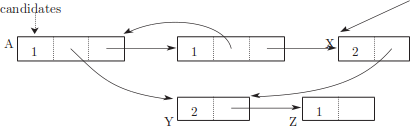
\includegraphics{figures/refcnt_2a}
    \caption{Πριν τη διαδικασία \textproc{markGrey}.}
  \end{subfigure}

  \begin{subfigure}[b]{1.0\textwidth}
    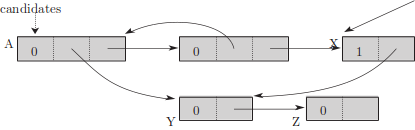
\includegraphics{figures/refcnt_2b}
    \caption
      {Μετά τη \textproc{markGrey}, όλα τα αντικείμενα που
       είναι προσβάσιμα από ένα αντικείμενο υποψήφιο μέλος
       κύκλου σκουπιδιών έχουν σημανθεί γκρι και η επίδραση
       των εσωτερικών δεικτών αυτού του γκρι υπογράφου έχει
       αφαιρεθεί. Ο μετρητής αναφορών του αντικειμένου $X$,
       το οποίο είναι ακόμη προσβάσιμο, έχει μη μηδενική
       τιμή.}
  \end{subfigure}
  
  \begin{subfigure}[b]{1.0\textwidth}
    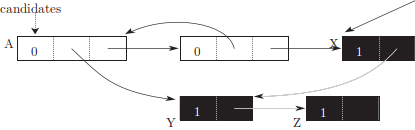
\includegraphics{figures/refcnt_2c}
    \caption
      {Μετά τη \textproc{scan}, όλα τα προσβάσιμα αντικείμενα
       είναι μαύρα και οι μετρητές αναφορών αυτών έχουν
       επιδιορθωθεί και αντικατοπτρίζουν ζωντανές αναφορές.}
  \end{subfigure}
  \caption[Κυκλική καταμέτρηση αναφορών.]
    {Κυκλική καταμέτρηση αναφορών. Το πρώτο πεδίο κάθε
     αντικειμένου αποθηκεύει το μετρητή αναφορών του.}
  \label{fig:refcnt_2}
\end{figure}

Στη δεύτερη φάση της συλλογής, εξετάζονται οι μετρητές
αναφορών κάθε αντικειμένου που είναι υποψήφια ρίζα ενός
κύκλου σκουπιδιών καθώς και των αντικειμένων που ανήκουν
στο μεταβατικό κλείσιμο αυτού ως προς την προσβασιμότητα
μέσω δεικτών. Αν ο μετρητής αναφορών ενός αντικειμένου
βρεθεί θετικός, τότε σίγουρα υπάρχει εξωτερική αναφορά
προς αυτό. Στην περίπτωση αυτή, η διαδικασία
\textproc{scanBlack} αναιρεί την επίδραση της διαδικασίας
\textproc{markGrey} αυξάνοντας το μετρητή αναφοράς και
χρωματίζοντας το αντικείμενο μαύρο. Αντίθετα, αν ο μετρητής
αναφορών είναι μηδενικός, η διαδικασία \textproc{scan}
χρωματίζει το αντικείμενο λευκό και εξετάζει αναδρομικά τα
παιδιά του. Στο σημείο αυτό δε μπορούμε με βεβαιότητα να
υποθέσουμε πώς ένα λευκό αντικείμενο είναι σκουπίδι, καθώς
αυτό μπορεί να επανεξετασθεί αργότερα από κλήση της
διαδικασίας \textproc{scanBlack} με όρισμα κάποιο άλλο
αντικείμενο του υπογράφου.

Τέλος, η τρίτη φάση, η οποία υλοποιείται από τη διαδικασία
\textproc{collectWhite} αποδεσμεύει τα λευκά αντικείμενα.
Επαναληπτικά, μέχρις ότου αδειάσει το σύνολο υποψηφίων ριζών
κύκλων σκουπιδιών αφαιρείται από αυτό ένα αντικείμενο και
εξετάζεται το χρώμα του. Αν είναι λευκό, το αντικείμενο
ελευθερώνεται (χρωματίζεται μαύρο) και στη συνέχεια
εξετάζονται αναδρομικά τα παιδιά του. Η διαδικασία
\textproc{collectWhite} δεν επεξεργάζεται αντικείμενα
παιδιά που τυχαίνει να βρίσκονται στο σύνολο των υποψηφίων
ριζών κύκλων σκουπιδιών: η ελευθέρωσή τους πραγματοποιείται
σε επόμενη επανάληψη του βρόχου της διαδικασίας
\textproc{collectCandidates}.

Ο αλγόριθμος Recycler μπορεί να βελτιστοποιηθεί περαιτέρω με
την στατική αναγνώριση πώς αντικείμενα συγκεκριμένων κλάσεων
δε μπορούν να είναι μέλη κύκλων σκουπιδιών (όπως για παράδειγμα
αντικείμενα που δεν περιέχουν δείκτες, αλλά όχι μόνο) και
ως εκ τούτου δε χρειάζεται να μπουν στο σύνολο των υποψήφιων
ριζών κύκλων σκουπιδιών. Τα αντικείμενα αυτά χρωματίζονται
πράσινα και όχι μαύρα. Οι Bacon και Rajan
\cite{DBLP:conf/ecoop/BaconR01} διαπιστώνουν πώς αυτή η
βελτιστοποίηση μειώνει κατά μία τάξη μεγέθους το μέγεθος
του συνόλου υποψηφίων ριζών κύκλων σκουπιδιών. 

\section{Ανακεφαλαίωση και θέματα προς εξέταση}
Η καταμέτρηση αναφορών είναι ελκυστική για την προθυμία
συλλογής αντικειμένων σκουπιδιών αλλά και τις ιδιότητες
τοπικότητας αυτής. Η απλοϊκή καταμέτρηση αναφορών μπορεί
να ανακτήσει τη μνήμη από ένα αντικείμενο αμέσως μόλις
αφαιρείται ο τελευταίος δείκτης που αναφέρεται σε αυτό.
Η λειτουργία της εμπλέκει μόνο τους παλαιούς και νέους
στόχους των δεικτών που εγγράφονται ή διαβάζονται, σε
αντίθεση με τη συλλογή εξιχνίασης που επισκέπτεται κάθε
ζωντανό αντικείμενο στο σωρό. Ωστόσο, τα πλεονεκτήματα
της μεθόδου είναι ταυτόχρονα και τα μειονεκτήματα της.
Καθώς δεν μπορεί να ελευθερώσει ένα αντικείμενο μέχρις
ότου κανένας δείκτης δεν αναφέρεται σε αυτό, δεν μπορεί
να συλλέξει κύκλους σκουπιδιών. Επιπλέον, προσθέτει ένα
μικρό κόστος σε κάθε λειτουργία \textproc{Read} και
\textproc{Write} του τροποποιητή, επιβαρύνοντας με τον
τρόπο αυτό τη ρυθμαπόδοση του τελευταίου περισσότερο σε
σχέση με τη συλλογή εξιχνίασης. Επιπλέον, οι πολυνηματικές
εφαρμογές απαιτούν τον αυστηρό συγχρονισμό των τροποποιήσεων
των μετρητών αναφορών και των ενημερώσεων δεικτών. Τέλος,
η συλλογή σκουπιδιών με καταμέτρηση αναφορών αυξάνει το
μέγεθος των αντικειμένων.

\subsection{Περιβάλλον εκτέλεσης}
Παρά τα παραπάνω ζητήματα, ο αποκλεισμός της καταμέτρησης
αναφορών χωρίς περαιτέρω σκέψη είναι εσφαλμένος. Ασφαλώς
και δεν είναι κατάλληλη ως τμήμα του διαχειριστή μνήμης
μιας εικονικής μηχανής γενικού σκοπού, ειδικά αν τα
εμπλεκόμενα αντικείμενα είναι μικρά, εμφανίζονται συχνά
κύκλοι και ο ρυθμός λειτουργιών εγγραφής δεικτών από τον
τροποποιητή είναι υψηλός. Ωστόσο, υπάρχουν περιβάλλοντα
στα οποία η χρήση καταμέτρησης αναφορών είναι κατάλληλη.
Η καταμέτρηση αναφορών αποδεικνύεται αποδοτική σε
περιβάλλοντα όπου οι χρόνοι ζωής των περισσότερων
αντικειμένων είναι αρκετά απλοί ώστε αυτά να διαχειρίζονται
ρητώς. Μπορεί επίσης να περιορισθεί στη διαχείριση ενός
μικρότερου αριθμού πόρων με πιο σύνθετες σχέσεις
ιδιοκτησίας. Συχνά οι πόροι αυτοί είναι μεγάλα αντικείμενα
με αποτέλεσμα το κόστος της προσθήκης στην επικεφαλίδα μιας
λέξης για την αποθήκευση του μετρητή αναφοράς να είναι
αμελητέο. Δεδομένα όπως bitmaps ψηφιακών εικόνων δεν
περιλαμβάνουν δείκτες και συνεπώς είναι αδύνατη η εμφάνιση
κύκλων σκουπιδιών. Επιπρόσθετα, η καταμέτρηση αναφορών
μπορεί να υλοποιηθεί ως τμήμα μιας βιβλιοθήκης και όχι
ως τμήμα του συστήματος εκτέλεσης, δίνοντας με τον τρόπο
αυτό πλήρη έλεγχο στον προγραμματιστή όσον αφορά τη χρήση
της. Στην περίπτωση αυτή βέβαια απαιτείται ιδιαίτερη
προσοχή από τον προγραμματιστή, ο οποίος πρέπει να
εξασφαλίσει την απουσία καταστάσεων συναγωνισμού μεταξύ
λειτουργιών εγγραφής δεικτών και ενημερώσεων μετρητών
αναφορών.

\subsection{Προηγμένες τεχνικές}
Εξεζητημένοι αλγόριθμοι καταμέτρησης αναφορών προσφέρουν
λύσεις για τα περισσότερα από τα προβλήματα που αντιμετωπίζει
η απλοϊκή καταμέτρηση αναφορών, επιβάλλοντας ωστόσο παύση
του κόσμου, όπως συμβαίνει και στη συλλογή εξιχνίασης.

Η μνήμη αντικειμένων ενός κύκλου σκουπιδιών μπορεί να ανακτηθεί
από ένα εφεδρικό συλλέκτη εξιχνίασης, ή χρησιμοποιώντας την
τεχνική της δοκιμαστικής διαγραφής. Και στις δύο περιπτώσεις,
η εκτέλεση του τροποποιητή αναστέλλεται κατά τη διάρκεια
συλλογής των κύκλων σκουπιδιών.

Παρότι στη χειρότερη περίπτωση το πεδίο ενός αντικειμένου
όπου αποθηκεύεται ο μετρητής αναφορών πρέπει να είναι τόσο
μεγάλο ώστε να χωράει το μέγιστο πλήθος δεικτών, οι
περισσότερες εφαρμογές διατηρούν μικρό αριθμό αναφορών προς
τα περισσότερα αντικείμενα. Συχνά, είναι δυνατό να κλαπούν
μερικά bits από μια λέξη της επικεφαλίδας που χρησιμοποιείται
για την αποθήκευση ενός κλειδώματος ή ενός κωδικού
κατακερματισμού. Είναι βέβαια επίσης σύνηθες να υπάρχουν
πολλές αναφορές προς μερικά αντικείμενα.

Η επιβάρυνση στη ρυθμαπόδοση του τροποποιητή μπορεί να
μειωθεί παραλείποντας μερικές τροποποιήσεις δεικτών και
μειώνοντας το κόστος άλλων. Η καταμέτρηση αναφορών με
αναβολή αγνοεί τις εγγραφές από τον τροποποιητή των τοπικών
μεταβλητών. Αυτό επιτρέπει στους μετρητές αναφορών των
αντικειμένων που είναι προσβάσιμα από τις ρίζες να έχουν
μικρότερη τιμή από πραγματική και αποτρέπει την πρόωρη
ανάκτηση της μνήμης που αυτά καταλαμβάνουν. Η καταμέτρηση
αναφορών με συγκέντρωση λαμβάνει υπόψη την κατάσταση ενός
αντικειμένου μόνο στην αρχή και στο τέλος μιας εποχής,
αγνοώντας τις λειτουργίες εγγραφής δεικτών στο ενδιάμεσο
χρονικό διάστημα. Κατά κάποιο τρόπο είναι μια αυτόματη
βελτιστοποίηση: αφαιρεί τις περιττές ενδιάμεσες
επιδιορθώσεις των μετρητών αναφορών. Ωστόσο και πάλι,
τόσο η καταμέτρηση αναφορών με αναβολή όσο και η καταμέτρηση
αναφορών με συγκέντρωση επιβάλλουν την παύση του κόσμου
για ένα χρονικό διάστημα ώστε να επιδιορθωθούν οι μετρητές
αναφορών. Επιπλέον, προσθέτουν μία επιβάρυνση στις
απαιτήσεις σε χώρο της απλοϊκής καταμέτρησης αναφορών
για την αποθήκευση είτε του πίνακα μηδενικών μετρητών
αναφορών είτε των απομονωτών καταγραφής ενημερώσεων.

Ένα επιπρόσθετο πλεονέκτημα των προηγμένων αυτών τεχνικών
συλλογής με καταμέτρηση αναφορών είναι πώς κλιμακώνουν
καλά με μεγάλους σωρούς. Το κόστος τους είναι ανάλογο
μόνο προς τον αριθμό των εγγραφών δεικτών και όχι του
όγκου των δεδομένων ζωντανών αντικειμένων.
\end{greek}
